
\begin{figure}[h!]
    \centering
    \caption{Estimates of the effect of the minimum wage on rents, 
             Zillow rental index}
    \label{fig:dynamic_zori}

    \begin{subfigure}{.65\textwidth}
        \caption{Control for year-month by CBSA fixed effects}
        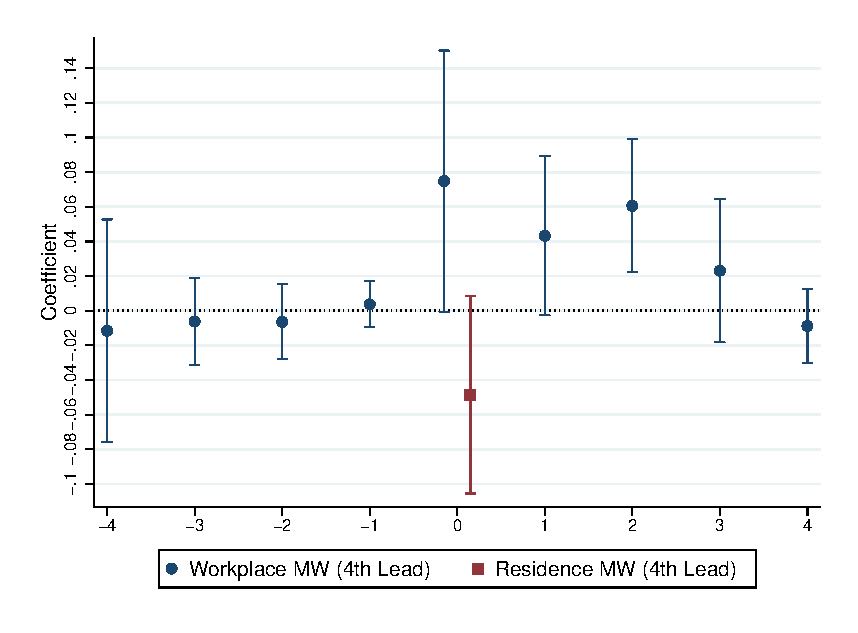
\includegraphics[width = 1\textwidth]
            {fd_zori/output/cbsa_time_FE}
    \end{subfigure}\\
    \begin{subfigure}{.65\textwidth}
        \caption{Control for year-month fixed effects}
        \includegraphics[width = 1\textwidth]
            {fd_zori/output/time_FE}
    \end{subfigure}

    \begin{minipage}{.95\textwidth} \footnotesize
        \vspace{3mm}
        Notes:
        Data are from the baseline estimation sample described in Section 
        \ref{sec:data_final_panel}.
        The figures show coefficients from regressions of the change in 
        log of Zillow rental index on leads and lags of the change in the 
        workplace MW and the change in the residence MW, using the 
        4th lead of the MW-based measures.
        The top panel includes CBSA by year-month fixed effects, whereas
        the bottom panel includes year-month fixed effects.
        Both regressions include economic controls that vary at the county by 
        month and county by quarter levels, which include the change of the 
        following variables: the log of the average wage, the log of employment, 
        and the log of the establishment count for the sectors 
        ``Information,'' ``Financial activities,'' and ``Professional and 
        business services.''
        95\% pointwise confidence intervals are obtained from standard errors 
        clustered at the state level.
    \end{minipage}
\end{figure}
